\documentclass[a4paper,11pt]{article}
\usepackage[utf8]{inputenc}
\usepackage[MeX]{polski}
\usepackage{hyperref}
\usepackage{graphicx}
\usepackage{pdfpages}
\usepackage{tikz}
\usepackage{fancyvrb}
\usepackage{rotating}
\usepackage{multirow}
\usepackage{amsmath}
\usepackage{amsfonts}
\usetikzlibrary{positioning,shapes,shadows,arrows}

\author{Michał Aniserowicz \href{mailto:michalaniserowicz@gmail.com}{{\small \nolinkurl{<michalaniserowicz@gmail.com>}}} \\ Jakub Turek \href{mailto:jkbturek@gmail.com}{{\small \nolinkurl{<jkbturek@gmail.com>}}}}
\title{{\Large [SAG.A] Dokumentacja końcowa projektu} \\ Protokół MAS z~wykorzystaniem ontologii}
\date{2 czerwca 2013r.}

\begin{document}

\maketitle

\section{Temat projektu}

Tematem projektu jest implementacja protokołu wykorzystującego ontologię w~systemie wieloagentowym. W ramach projektu opracowana została symulacja ruchu drogowego w~kwadratowej sieci ulic przypominającej plan Manhattanu. Symulacja składa się z~następujących elementów:


\begin{description}
    \item[miasto] określa ilość przecznic (wielkość przestrzeni),
    \item[kodeks ruchu drogowego] definiuje zasady poruszania się na drodze,
    \item[sygnalizacja świetlna] określa pierwszeństwo na części skrzyżowań,
    \item[samochód] porusza się po mieście zgodnie z~zasadami ruchu drogowego znajdującymi się w~kodeksie.
\end{description}

Projekt obejmuje również przygotowanie graficznego interfejsu użytkownika, który pełni dwojaką funkcję:

\begin{itemize}
    \item ukazuje aktualny stan miasta w~rzucie z~góry,
    \item pozwala na dynamiczną zmianę kodeksu ruchu drogowego.
\end{itemize}

\section{Technologia}

Projekt został zaimplementowany na platformie JADE\footnote{Java Agent DEvelopment Framework - \href{http://jade.tilab.org}{jade.tilab.org}.}. Interfejs graficzny został stworzony z~użyciem natywnych bibliotek języka Java (AWT oraz Swing). Implementacja tworzona była w~środowisku Eclipse i~testowana w~systemie operacyjnym Windows 7 64-bit.

\section{Agenci}

W~systemie zdefiniowanych jest pięć typów agentów:

\begin{description}
    \item[Miasto] określa rozmiar (w~przecznicach) siatki miasta. Posiada zachowania umożliwiające sprawdzanie, w~których kierunkach można przemierzyć skrzyżowanie w~określonej lokalizacji. Zakłada się, że w~jednym systemie symulacji występuje wyłącznie jeden agent miasta.
    \item[Kodeks ruchu drogowego] określa następujące przepisy ruchu:
        \begin{itemize}
            \item stronę jezdni, którą poruszają się samochody,
            \item pierwszeństwo samochodu w~zależności od jego typu,
            \item kolor sygnalizacji świetlnej oznaczający, że można wjechać na skrzyżowanie,
            \item wzajemne pierwszeństwo samochodów w~sytuacji, gdy na skrzyżowaniu nie ma sygnalizacji świetlnej.
        \end{itemize}
        
        Zakłada się, że w~jednym systemie symulacji występuje wyłącznie jeden agent kodeksu ruchu drogowego.
    \item[Samochód] agent poruszający się po mieście. Posiada własną funkcję celu, która zmienia się wraz z~upływem czasu. Komunikuje się z~miastem, kodeksem ruchu drogowego, sygnalizatorami świetlnymi oraz innymi samochodami. Autonomicznie decyduje o~swoim zachowaniu, to znaczy, że powinien (ale nie musi) respektować przepisy ruchu drogowego zdefiniowane w~kodeksie. Porusza się w~dziedzinie dyskretnej (skokowo), lecz w~sposób płynny (wielostopniowe przejeżdżanie przez przecznicę). Występowanie agenta jest opcjonalne, dowolna jest liczba jego instancji w~jednym systemie.
    \item[Sygnalizator świetlny] steruje ruchem na skrzyżowaniu. Posiada dwa stany opisujące aktualny kolor (czerwony lub zielony), które ulegają cyklicznej zmianie. Reprezentuje grupę sygnalizatorów dla danego skrzyżowania (od dwóch do czterech, w~zależności od liczby przecinających się na skrzyżowaniu jezdni). Występowanie agenta jest opcjonalne, dowolna jest liczba jego instancji w~jednym systemie.
    \item[Mapa miasta] odwzorowywuje, rzutem z~góry, stan miasta w~danej chwili czasu. Komunikuje się z~samochodami oraz sygnalizatorami świetlnymi, odpytując cyklicznie stan agentów. Występowanie agenta jest opcjonalne, dowolna jest liczba jego instancji w~jednym systemie.
\end{description}

\section{Ontologia}

Wykorzystanie ontologii umożliwiło opisanie zmiennych zasad ruchu drogowego, do których stosują się samochody. Ontologia jest wykorzystywana głównie przez trzy typy agentów:

\begin{description}
    \item[Samochód] nie zna autonomicznie topologii miasta. Stosuje się do obowiązujących zasad ruchu drogowego narzuconych przez kodeks.
    \item[Miasto] posiada informację, w~których kierunkach można przejechać przez dane skrzyżowanie.
    \item[Kodeks ruchu drogowego] posiada informacje o~obowiązujących przepisach ruchu drogowego.
\end{description}

\subsection{Koncepcje}

Tabela \ref{tab:concepts} przedstawia koncepcje zdefiniowane w~ontologii ruchu drogowego.

\begin{table}[ht!]
    \centering
    \begin{tabular}{|c|c|c|c|}
        \hline
        \multirow{2}{*}{\textbf{Koncepcja}} & \multicolumn{3}{|c|}{\textbf{Parametr}} \\
        \cline{2-4}
        & \textbf{Nazwa} & \textbf{Typ} & \textbf{Dozwolone wartości} \\
        \hline
        \multirow{2}{*}{Pozycja} & Współrzędna $x$ & Integer & $[0;city\_size)$ \\
        \cline{2-4}
        & Współrzędna $y$ & Integer & $[0;city\_size)$ \\
        \hline
        \multirow{4}{*}{Kierunek} & \multirow{4}{*}{Kierunek} & \multirow{4}{*}{Integer} & $0$ (północ), \\
        &&& $1$ (wschód), \\
        &&& $2$ (południe), \\
        &&& $3$ (zachód) \\
        \hline
        \multirow{8}{*}{Samochód} & Pozycja & Pozycja & - \\
        \cline{2-4}
        & Kierunek & Kierunek & - \\
        \cline{2-4}
        & \multirow{2}{*}{Typ} & \multirow{2}{*}{Integer} & $0$ (normalny), \\
        &&& $1$ (uprzywilejowany), \\
        \cline{2-4}
        & \multirow{3}{*}{Status} & \multirow{3}{*}{Integer} & $0$ (jedzie), \\
        &&& $1$ (przed skrzyżowaniem), \\
        &&& $2$ (na skrzyżowaniu) \\
        \hline
        \multirow{9}{*}{Sygnalizacja} & Pozycja & Pozycja & - \\
        \cline{2-4}
        & Kolor światła & \multirow{2}{*}{Integer} & $0$ (czerwone), \\
        & (północ) & & $1$ (zielone) \\
        \cline{2-4}
        & Kolor światła & \multirow{2}{*}{Integer} & $0$ (czerwone), \\
        & (wschód) & & $1$ (zielone) \\
        \cline{2-4}
        & Kolor światła & \multirow{2}{*}{Integer} & $0$ (czerwone), \\
        & (południe) & & $1$ (zielone) \\
        \cline{2-4}
        & Kolor światła & \multirow{2}{*}{Integer} & $0$ (czerwone), \\
        & (zachód) & & $1$ (zielone) \\
        \cline{2-4}
        \hline
    \end{tabular}

    \caption{Koncepcje zdefiniowane w~ontologii ruchu drogowego.}
    \label{tab:concepts}
\end{table}

\subsection{Predykaty}
\label{sec:predicates}

Samochody komunikują się z~innymi agentami głównie przy użyciu predykatów. Tabela \ref{tab:predicates} przedstawia zdefiniowane w~ontologii miasta predykaty.

\begin{table}[ht!]
    \centering
    \begin{tabular}{|c|c|c|c|}
        \hline
        \multirow{3}{*}{\textbf{Predykat}} & \multicolumn{3}{|c|}{\textbf{Parametr}} \\
        \cline{2-4}
        & \multirow{2}{*}{\textbf{Nazwa}} & \multirow{2}{*}{\textbf{Typ}} & \textbf{Dozwolone} \\
        &&& \textbf{wartości} \\
        \hline
        Czy można & Pozycja skrzyżowania & Pozycja & - \\
        \cline{2-4}
        skręcić? & Kierunek & Kierunek & - \\
        \hline
        Czy można & \multirow{2}{*}{Kolor światła} & \multirow{2}{*}{Integer} & $0$ (czerwone), \\
        przejechać? &&& $1$ (zielone) \\
        \hline
        Czy ma & \multirow{2}{*}{Samochód} & \multirow{2}{*}{Samochód} & - \\
        pierwszeństwo? &&& \\
        \hline
        Czy ma & Pozycja 1 & Pozycja & - \\
        \cline{2-4}
        pierwszeństwo? & Pozycja 2 & Pozycja & \\
        \hline
        Czy jeździ & \multirow{2}{*}{Strona} & \multirow{2}{*}{Integer} & $0$ (lewa), \\
        po stronie? &&& $1$ (prawa) \\
        \hline
    \end{tabular}

    \caption{Predykaty zdefiniowane w~ontologii ruchu drogowego.}
    \label{tab:predicates}
\end{table}

W~dziedzinie predykatów, algorytm przejeżdżania przez skrzyżowanie można przedstawić następująco:

\begin{enumerate}
    \item Sprawdź, w~jakich kierunkach można pokonać skrzyżowanie. Prześlij do miasta predykat ,,czy można skręcić?'' z~niewiadomą typu kierunek, wypełniając jednocześnie pozycję skrzyżowania, przez które chcesz przejechać. Oczekuj na listę predykatów, które spełniają zadany warunek.
    \item Sprawdź, czy Twój samochód posiada bezwzględne pierwszeństwo. Prześlij do kodeksu ruchu drogowego predykat ,,czy ma pierwszeństwo?'' z~pojedynczym parametrem i~oczekuj na potwierdzenie jego prawdziwości.
        
        \begin{enumerate}
            \item Jeżeli predykat jest prawdziwy, wjedź na skrzyżowanie i~zakończ algorytm.
            \item Jeżeli predykat nie jest prawdziwy, kontynuuj algorytm.
        \end{enumerate}
        
    \item Sprawdź, czy na skrzyżowaniu znajdują się światła. Jeżeli nie, kontynuuj algorytm od kolejnego punktu. Jeżeli tak, sprawdź kolor świateł i~wyślij do kodeksu ruchu drogowego predykat ,,czy można przejechać?'' uzupełniony kolorem światła. Oczekuj na potwierdzenie spełnienia predykatu.
        
        \begin{enumerate}
            \item Jeżeli predykat jest prawdziwy, wjedź na skrzyżowanie i~zakończ algorytm.
            \item Jeżeli predykat nie jest prawdziwy, kontynuuj algorytm.
        \end{enumerate}
        
    \item Sprawdź, czy w~pobliżu skrzyżowania znajdują się inne samochody. Jeżeli nie, wjedź na skrzyżowanie i~zakończ algorytm. Jeżeli tak, dla każdego samochodu wypełnij predykat ,,czy ma pierwszeństwo?'' z~dwoma parametrami i~oczekuj na potwierdzenie jego prawdziwości.
        
        \begin{enumerate}
            \item Jeżeli wszystkie predykaty są fałszywe, wjedź na skrzyżowanie i~zakończ algorytm.
            \item Jeżeli chociaż jeden z~predykatów jest prawdziwy, oczekuj na przejechanie samochodu przez skrzyżowanie, a~następnie powtórz algorytm od punktu 4.
        \end{enumerate}
\end{enumerate}

\section{Protokół}

Wykorzystywany w~symulacji ruchu ulicznego protokół został przybliżony razem z~algorytmem opartym na predykatach w~sekcji \ref{sec:predicates}. Na następnej stronie przedstawiony jest jego większy fragment, który jest inicjowany ze strony samochodu przed wjazdem na skrzyżowanie.



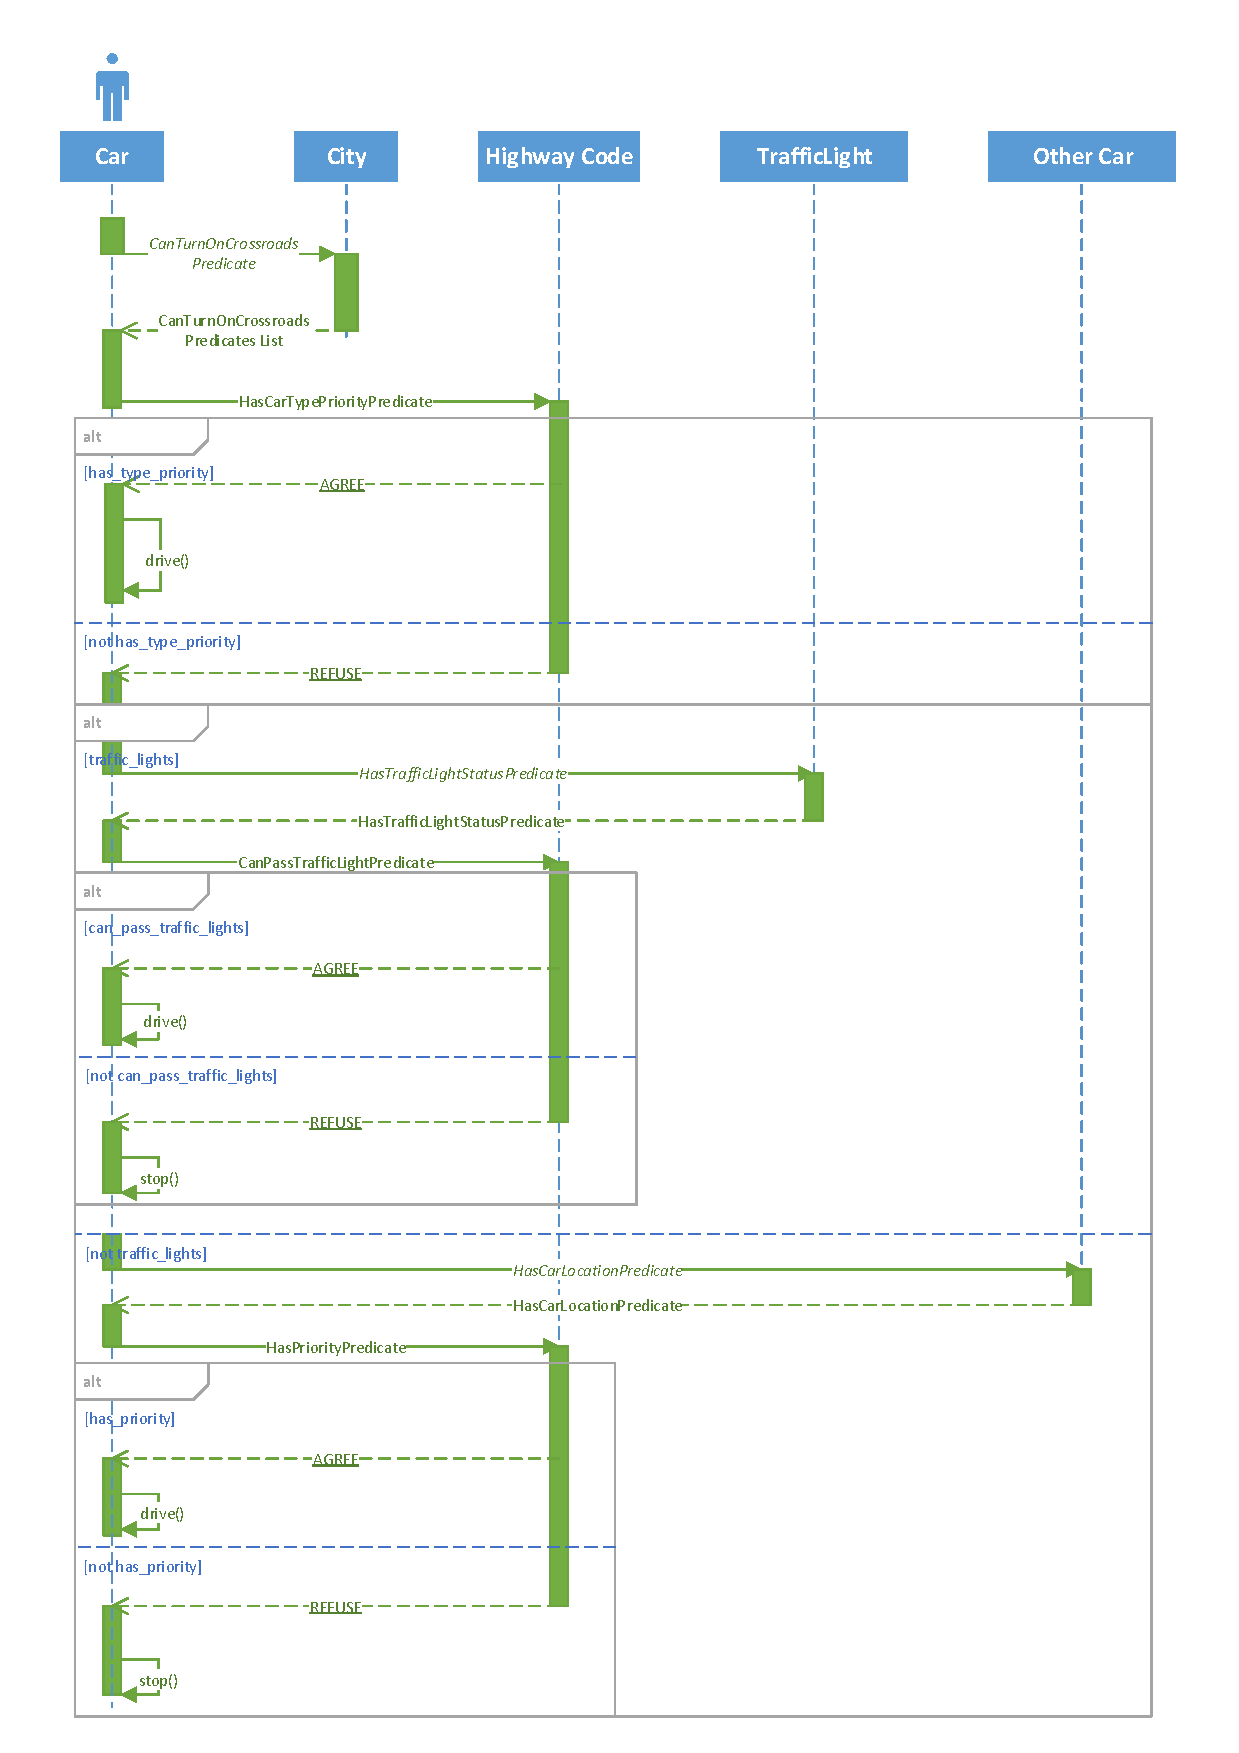
\includepdf{protocol.pdf}

\end{document}